\chapter{Episode Mining Background}
\label{chapter_background}

% **************************** Define Graphics Path **************************
\ifpdf
    \graphicspath{{Chapter3/Figs/Raster/}{Chapter3/Figs/PDF/}{Chapter3/Figs/}}
\else
    \graphicspath{{Chapter3/Figs/Vector/}{Chapter3/Figs/}}
\fi

This chapter establishes the terminology and basic formal definitions for this thesis. While episodes were already intuitively defined and talked about in the previous chapters it is important to formally define episodes, since formal definitions are clear and unambiguous. This is helpful in order to define and explain mining objectives and techniques as well as algorithms that are used in this thesis. 

\section{Basic Definitions}
\label{sec_basicEpisodeDefinitions}
Episodes are complex events whose basic building blocks are simple events. Note that in order to make use of episodes it is necessary that all simple events have a type and there is a finite, previously known event alphabet, that contains these types. In this thesis the event alphabet is referred to as $\Sigma$. Formally episodes are defined in the following way:

\begin{mydef}
\label{def_episode}
\textbf{Episode} An episode (also sometimes called episode pattern or elementary episode) $\alpha$ of length $m$ (also called m-episode) is defined as a triple: $\alpha = (V_\alpha,{\leq}_{\alpha},g_\alpha)$ where $V_\alpha = \{v_1,...,v_m\}$ is a set of nodes, ${\leq}_{\alpha}$ is a partial order over $V_\alpha$ and $g_\alpha : V_\alpha \rightarrow \Sigma$ is a mapping that maps each node of $V_\alpha$ to an event type. \cite{mannila1995discovering}
\end{mydef}

Put more simply an episode is a multiset of event types, whose elements can be, but do not have to be ordered by a relation (${\leq}_{\alpha}$). Another way of putting it is that an episode is essentially a partially ordered sequence of events. Before examples are studied there are a two special types of episodes that need to be mentioned since they have received the most attention in the available literature. These are called serial and parallel episodes:

\begin{mydef}
\label{def_serialEpisode}
\textbf{Serial Episode} An episode $\alpha = (V_\alpha,{\leq}_{\alpha},g_\alpha)$ is called a serial episode if ${\leq}_{\alpha}$ is a total order. \cite{mannila1995discovering}
\end{mydef}

\begin{mydef}
\label{def_parallelEpisode}
\textbf{Parallel Episode} An episode $\alpha = (V_\alpha,{\leq}_{\alpha},g_\alpha)$ is called a parallel episode if ${\leq}_{\alpha} = \emptyset$, in other words if there is no ordering imposed on $V_\alpha$ at all. \cite{mannila1995discovering}
\end{mydef}

Essentially, serial episodes are sequences, while parallel episodes are multisets. Figure \ref{fig_exampleEpisodes} visualizes example episodes as directed acyclic graphs (DAG).

\begin{figure}[h]
	\centering
  	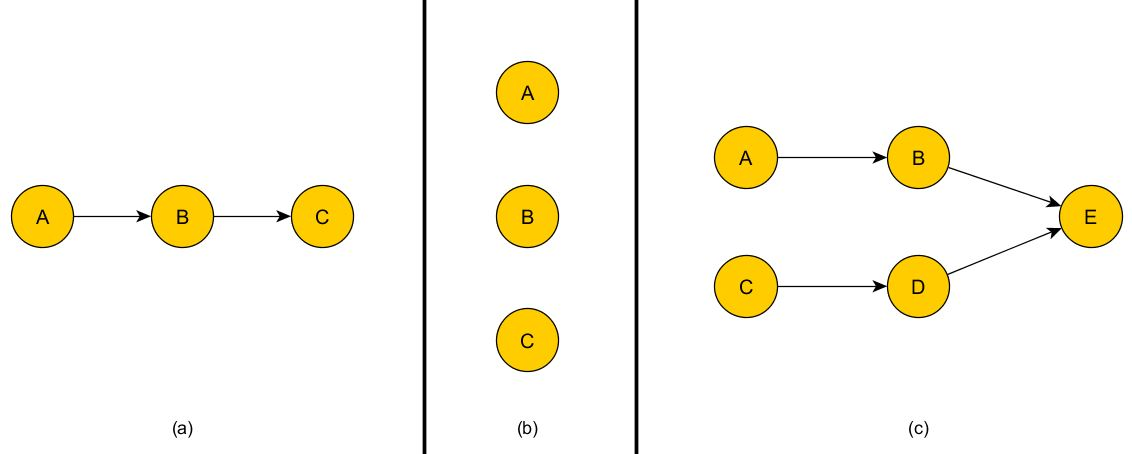
\includegraphics[width=\textwidth]{exampleEpisodes}
	\caption{An example of different episodes: (a) - a serial episode, (b) - a parallel episode, (c) - an elementary (composite) episode}
	\label{fig_exampleEpisodes}
\end{figure}

%\begin{figure}[H]
%\centering
%\begin{tabular}{c|c|c}
%\begin{subfigure}{.3\textwidth}
%  \centering
%  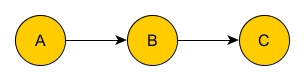
\includegraphics[width=\linewidth]{exampleSerialEpisode}
%  \caption{A serial episode}
%  \label{fig:sub1}
%\end{subfigure}%
%&
%\begin{subfigure}{.3\textwidth}
%  \centering
%  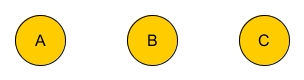
\includegraphics[width=\linewidth]{exampleParallelEpisode}
%  \caption{A parallel episode}
%  \label{fig:sub2}
%\end{subfigure}
%&
%\begin{subfigure}{.3\textwidth}
%  \centering
%  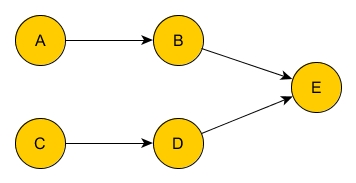
\includegraphics[width=\linewidth]{exampleCompositeEpisode}
%  \caption{An elementary (composite) episode}
%  \label{fig:sub3}
%\end{subfigure}
%\end{tabular}
%\caption{Different example episodes visualized as directed acyclic graphs}
%\label{fig_exampleEpisodes}
%
%\end{figure}

In fact each episode can be formally transformed to a DAG using the following simple procedure: Given an Episode $\alpha = (V_\alpha,{\leq}_{\alpha},g_\alpha)$, create the corresponding DAG $G = (V,E)$ by executing the following:

\begin{enumerate}
	\item For each $v \in V_\alpha$ add $v$ to $V$ and label $v$ with $g_\alpha (v)$
	\item For each pair $v,w \in V_\alpha$ where $v \, {\leq}_{\alpha} \, w $ add edge $(v,w)$ to $E$
\end{enumerate}

The original paper by Manilla et al. \cite{mannila1995discovering} also introduces the notion of composite episodes:

\begin{mydef}
\label{def_compositeEpisodes}
\textbf{Composite Episode} An episode $\alpha = (V_\alpha,{\leq}_{\alpha},g_\alpha)$ is called a composite episode if $g_\alpha : V_\alpha \rightarrow \Sigma \cup C^*$, where $C^*$ is the set of all composite episodes. \cite{mannila1995discovering}
\end{mydef}

This recursive definition of composite episodes may be confusing at first, since it is formulated very compactly. A slightly more clear way to look at it is the following:\\
A composite episode is either:
\begin{itemize}
	\item A single event (An elementary episode of length 1).
	\item A serial composition of two composite episodes
	\item A parallel composition of two composite episodes
\end{itemize}

This definition has the advantage that any elementary episode can be represented as a composite episode which is exclusively a serial or parallel composition of serial, parallel or composite subepisodes (see definition \ref{def_subEpisode}). Note that composite episodes are not more expressive than elementary episodes as defined in definition \ref{def_episode}, it is just a recursive way of defining episodes. \\
Interestingly, there are other parts of the related work that use the term \textit{composite episodes} but deviate from definition \ref{def_compositeEpisodes}. For example Baathorn et al. propose a method for finding composite episodes \cite{bathoorn2007finding}. However they define composite episodes as a sequence of parallel episodes, which is more restrictive than the original definition. Also Baumgarten et al. use this definition \cite{baumgarten2003tree} when they present an approach to mine descriptive composite episodes. Note that not all elementary episodes can be represented as sequences of parallel episode. A simple example shown in figure \ref{fig_notSequenceOfSet} illustrates this.

\begin{figure}[h]
	\centering
  	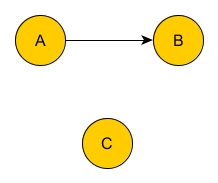
\includegraphics[width=0.3\textwidth]{notSequenceOfSet}
	\caption{An elementary episode that can not be represented as a sequence of parallel episodes}
	\label{fig_notSequenceOfSet}
\end{figure}

If the presented episode were to be represented as a sequence of parallel episodes obviously $A$ and $B$ would have to be in different parallel episodes in order to fulfill the requirement that $B$ must be after $C$. After that the problem is that it is impossible to assign $C$ to any of those sets. If it gets assigned to the same parallel episode set as $A$ then this would prohibit $A$ and $B$ occurring first followed by $C$, which is allowed in the original definition. Likewise if $C$ gets assigned to the same parallel episode as $B$ then that eliminates the possibility of $C$ occurring before $A$ and $B$, which once again was allowed in the elementary episode. It should also be noted that some authors simply refer to serial episodes as episodes, which leads to somewhat of a blurry terminology across the research area. For this thesis I stick to the original terminology as defined in definitions to \ref{def_episode} to \ref{def_compositeEpisodes}. \newline
If I want to quickly denote simple episodes formally without drawing a DAG, I will use $\rightarrow$ as the sequence (ordering) operator. To show that there is no order specified between two nodes I use $\|$ as the parallel operator. For example $(A \, \| \, B ) \rightarrow C$ denotes a composite episode of length 3, which specifies that it does not matter in which order $A$ or $B$ occur, but $C$ must occur after both $A$ and $B$. If more complex episodes need to be discussed they will be visualized as directed acyclic graphs like in the previous figures. \newline 
In algorithms the following notation is used to access episodes:

\begin{itemize}
	\item for all episodes $\alpha = (V_\alpha,{\leq}_{\alpha},g_\alpha)$ the term $|\alpha | = |V_\alpha|$ is used to denote the length of the episode.
	\item for serial episodes $\alpha [i]$ refers to the event type of the i-th node of $\alpha$ with respect to the total ordering imposed on $\alpha$ by ${\leq}_{\alpha}$. In other words $\alpha [i]$ is the i-th element of the sequence of event types, defined by the serial episode $\alpha$.
	\item for parallel episodes $\alpha$ the condition $E \in \alpha$ holds if there is at least one $v \in V_\alpha$, so that $g_\alpha(v) = E$. In this context let $count(\alpha,E)= |\{v \in V_\alpha \mid g_\alpha(v) = E\}|$, meaning $count(\alpha,E)$ is the number of nodes in the parallel episode $\alpha$ that have type $E$.
\end{itemize}

The notion of sub- and superpatterns, which is very important for most pattern mining applications also applies to episodes, as shown in the next definition.

\begin{mydef}
\label{def_subEpisode}
\textbf{Subepisode} An episode $\beta = (V_\beta,{\leq}_{\beta},g_\beta)$ is said to be a subepisode of episode $\alpha = (V_\alpha,{\leq}_{\alpha},g_\alpha)$ if all of the following conditions hold:
\begin{enumerate}
	\item The nodes of $\beta$ are a subset of the nodes of $\alpha$: \\
	$V_\beta \subseteq V_\alpha$
	\item All nodes of $\beta$ are assigned to the same event type as their corresponding nodes in $\alpha$:\\
	 $\forall v \in V_\beta \; : \; g_{\beta}(v) = g_\alpha (v) $
	\item The ordering in $\alpha$ is at least as strict as the ordering in $\beta$:\\
	$\forall v,w \in V_\beta \, , v \, {\leq}_{\beta} \, w \; : \; v \, {\leq}_{\alpha} \, w$
\end{enumerate}
In this context $\alpha$ is also called the superepisode of $\beta$. \cite{mannila1995discovering,laxman2007fast}.
\end{mydef}

It is important to note that in the original definition of sub- and superepisodes by Mannila et al. \cite{mannila1995discovering}, the first property of the above definition was actually defined as $V_\beta \subset V_\alpha$, which implies that subepisodes would always have to consist of at least one less node than their superepisodes. This definition was changed by Laxman et al. \cite{laxman2007fast} to allow set equality as well. The implications of this change are that parallel episodes like $A \| B$ are now subepisodes of their serial counterparts of the same length $A \rightarrow B$. In this thesis I stick to the definition that allows set equality between super- and subepisodes. In both cases however subepisodes may relax the ordering specified in their superepisodes. For example if given the serial episode $\alpha =( A \rightarrow B \rightarrow C )$, not only $A \rightarrow B$ is a subepisode of $\alpha$ but also $A \| B$. \\
So far I have introduced a lot about episode patterns but it is not yet clear how episodes patterns occur in data. It is helpful to think of the episode patterns defined above as templates for concrete occurrences. In order to define what is meant by an episode occurrence, it is necessary to formally introduce the notion of an event sequence.

\begin{mydef}
\label{def_eventSequence}
\textbf{Event sequence} An event sequence is defined as an ordered list of tuples $S = [ (T_1,t_1),..., (T_n,t_n) ] $ where $T_i \in \Sigma$ is the event type of the i-th event and $t_i \in \mathbb{N}^+$ is the timestamp of the i-th event. The sequence is ordered according to the timestamps, which means that $\forall i,j \in \{1,...,n\} \; i<j \implies t_i \leq t_j$. \cite{mannila1997discovery} 
\end{mydef}

Note that it is allowed for two or more consecutive elements in a sequence to have the same timestamp. This is necessary in order to allow for multiple events to occur at the same time. The ordering of events with the same timestamp is not further specified and irrelevant in most cases. Another way to define such sequences is to define them as sequences of event sets in which consecutive event sets must all have different timestamps and events that occur simultaneously are part of the same set \cite{bathoorn2007finding}. Definitions from other authors explicitly prohibit two events happening at the same time \cite{baumgarten2003tree}. Which definition is appropriate depends on the context, for this thesis I will stick with definition \ref{def_eventSequence}. \\
Given the notion of an event sequence episode occurrences can now be defined:

\begin{mydef}
\label{def_episodeOccurrence}
\textbf{Episode Occurrence} An event episode $\alpha = (V_\alpha,{\leq}_{\alpha},g_\alpha)$ is said to occur in a sequence $S$ if events of the types that the nodes in $V_\alpha$ are mapped to by $g_\alpha$, occur in $S$ in the same order that they occur in the episode. More formally if given a sequence of events $S=[(T_1,t_1),...,(T_n,t_n)]$ an occurrence of $\alpha$ is defined as an injective Map $h:V_\alpha \rightarrow \{1,...,n\}$, where $g_\alpha (v) = T_{h(v)}$ and $\forall \, v,w \in V_\alpha : v \;{\leq}_{\alpha}\; w \implies t_{h(v)} \le t_{h(w)}$ holds. \cite{mannila1995discovering}
\end{mydef}

An episode pattern in itself does not specify any time span in which the events of the episode must occur, however if given an episode occurrence the duration of that occurrence can be defined. Durations of episode occurrences become relevant in practical applications, when the user wants to forbid episode occurrences that range over a time period that is too large. 

\begin{mydef}
\label{def_episodeOccurrence}
\textbf{Episode Occurrence Duration} The duration of an occurrence is defined as the difference between the timestamps of the last and first event that the episode nodes are mapped to. More formally if given an episode $\alpha$, a sequence $S=[(T_1,t_1),...,(T_n,t_n)]$ and an occurrence $h:V_\alpha \rightarrow \{1,...,n\}$ the episode duration is defined as $t_{last} - t_{first}+1$, where $last = max( \{h(v)| v \in V_\alpha \}$ and $first = min( \{h(v)| v \in V_\alpha \}$.
\end{mydef}

An example of an episode pattern, a sequence and two occurrences is visualized in figure \ref{fig_occurrenceExample}.

\begin{figure}[h]
	\centering
  	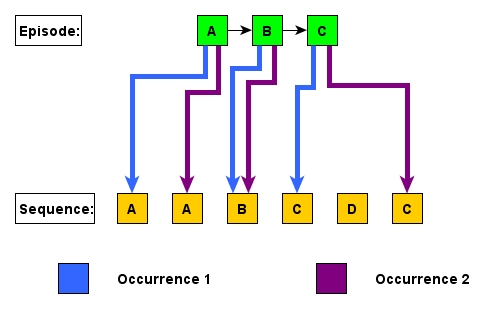
\includegraphics[width=\textwidth]{occurrenceExample}
	\caption{A visualization of the concept of episode occurrences in an event sequence. The episode pattern is drawn in green, the sequence in yellow. An occurrence is defined as a mapping from the nodes of the pattern to events in the sequence (see definition \ref{def_episodeOccurrence}). Thus the occurrences are visualized as arrows of different colors (blue and purple). }
	\label{fig_occurrenceExample}
\end{figure}


\section{Episode Discovery and General Mining Algorithm}
\label{sec_episodeDiscovery}
When discovering episodes in a sequence one is usually interested in those episodes that occur frequently, meaning more often than a user defined threshold. This is similar to the classical pattern mining algorithms, such as the apriori algorithm for finding frequent itemsets \cite{agrawal1994fast}. The apriori algorithm utilizes a principle that has become known as the apriori principle. The apriori-principle states that if a pattern is frequent, then all of its sub-patterns must be frequent as well. With the help of this knowledge the search space of all potential patterns can be pruned, since only those patterns, whose sub-patterns are all frequent, need to be considered. A general algorithm for mining the episodes occurring frequently in a sequence is given in algorithm \ref{alg_generalEpisodeMining}. The algorithm is very alike the basic apriori algorithm, since it uses a level-wise, breadth first search by first identifying all frequent episodes of a certain length $i$ and then uses these frequent episodes to generate candidates (possibly frequent episodes) of length $i+1$. In order for this to be correct, episode frequency must of course fulfill the apriori principle \cite{agrawal1994fast}. Intuitively one would assume that this is always true for episodes but strictly speaking this depends on the definition of episode frequency. However, any frequency definition of episodes that does not satisfy the apriori principle would be highly questionable to say the least, since this would eliminate the possibility of an efficient candidate generation that prunes those episodes which have infrequent subepisodes. To the best of the author's knowledge all frequency definitions proposed in the literature satisfy the apriori principle.\newline

\begin{algorithm}[H]
  \caption{General mining algorithm for frequent episodes
    \label{alg_generalEpisodeMining}}
  \begin{algorithmic}[1]
    \Statex
    \Function{EpisodeMining}{}
      \Let{$C_i$}{Episodes of Length 1} 
      \Let{$freq$}{$\emptyset$}
      \Let{$i$}{$1$}
      \While{$C_i \neq \emptyset$}
      	\State Count frequencies of each Episode $E \in C_i$
        \Let{$L_i$}{ $\{ E \mid E \in C_i \land C_i \; is\; frequent\}$}
        \Let{$freq$}{$freq \cup L_i$}
        \Let{$C_{i+1}$}{Generate Episode Candidates of length $i+1$ from $L_i$}
        \Let{$i$}{$i+1$}
      \EndWhile
      \State \Return{$freq$}
    \EndFunction
  \end{algorithmic}
\end{algorithm}


In summary, the general mining algorithm for frequent episodes requires:

\begin{itemize}
	\item A definition of episode frequency, that does not violate the apriori principle
	\item An algorithm for counting episode frequency (of concrete candidates) according to this definition
	\item An algorithm to generate candidate episodes
\end{itemize}

It may be a bit confusing that a definition of episode frequency for such a mining algorithm is needed. Since it was already defined what an occurrence of an episode looks like it would seem that counting all occurrences of an episode would yield its frequency. While this is a possible definition of frequency, it is important to note that finding all occurrences of an episode within a sequence is neither practical nor useful. An example will demonstrate the problem with this. Consider the simple serial episode $A \rightarrow B$ and a sequence of length $2\cdot n$ which repeats the subsequence $(A,B)$ $n$ times. One quickly realizes that the number of episode occurrences is very large due to the possibility of overlapping episode occurrences. In this particular case there are already $ \frac{n \cdot (n+1)}{2}$ possible occurrences. This number swiftly increases with the length of the episode pattern, since it introduces more potential overlappings. Naturally the number of possible parallel and composite episode occurrences is even larger, since they are less restrictive in the order of the events. Additionally, such a frequency definition would violate the apriori principle, since subepisodes can have less occurrences than their superepisodes. Consider the example sequence $[A,B,C,A,B,C]$ (timestamp values are left out). In this sequence there are three distinct occurences for the episode $A \rightarrow B$ and four distinct occurrences for its superepisode $A \rightarrow B \rightarrow C$. These detrimental effects of this naive frequency definition are nicely summarized by Laxman et al. in a paper presenting the non-overlapped frequency definition \cite{laxman2007fast}. \newline
An extensive summary of all proposed frequency measures for episodes can be found in a paper by Achar et al. \cite{achar2012unified}. The most common frequency definitions for episodes will be dealt with in sections \ref{sec_windowBased} and \ref{sec_otherFrequency}. Each frequency definition comes with its own counting algorithm that determines the frequency of candidate episodes in a sequence. The procedure for generating candidates is independent of the frequency definition and is presented in section \ref{sec_candidateGen}. \newline


\section{Window Based Frequency}
\label{sec_windowBased}
The window based frequency was the first frequency definition for episodes to gain general popularity. It was conceived by Mannila et al. \cite{mannila1995discovering}, although the frequency counting algorithms were only mentioned in text form. The same authors  specified the algorithms in a later paper \cite{mannila1997discovery}, which acts as the primary source for the overview given in this subsection. In order to define the window based frequency the notion of a time window needs to be introduced: 

\begin{mydef}
\label{def_timeWindow}
\textbf{Time Window} Given a sequence of events $S$ we define the Time Window $W(S,q,r)$ with $q,r \in \mathbb{N}^+$ and $q < r$ as the ordered subsequence of $S$ that includes all events of the sequence $S$ that have a timestamp $t$ where $q \leq t\leq r$. We call $w = r-q+1$ the duration of Window $W$. We denote the size of the window, meaning the number of events in it as $|W|$.
\end{mydef}

An example of how windows of a fixed duration are located in a sequence of events is presented in figure \ref{fig_windowBasedFrequency}.

\begin{figure}[h]
	\centering
  	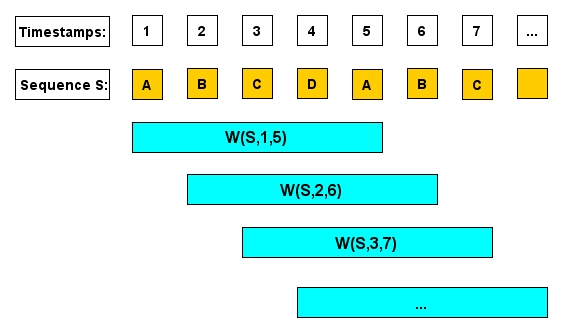
\includegraphics[width=\textwidth]{windowBasedFrequency}
	\caption{Different time windows of duration 5 in an event sequence.}
	\label{fig_windowBasedFrequency}
\end{figure}


\begin{mydef}
\label{def_windowBasedFrequency}
\textbf{Episode Frequency - Window based Definition} Given a sequence of events $S$, a fixed window duration of $w$ and an episode $\alpha$, we define the window based frequency $w\_freq(\alpha )$ as the number of windows $W$ with duration $w$ of $S$ in which $\alpha$ occurs: $w\_freq(\alpha ) = |\,\{W(S,q,r) \mid r-q+1 = w \land \alpha \;occurs\; in\; W \}\,|$.
\end{mydef}


For example given the sequence visualized in figure \ref{fig_windowBasedFrequency} $A \rightarrow B \rightarrow C$ occurs in windows $W(S,1,5)$ and $W(S,3,7)$. \newline 
This definition can be confusing at first since it is intended that episode occurrences that are comprised of the exact same events count just as many times as there are windows in which the events appear. In the previously mentioned example, we can find the episode $C \rightarrow D$ in the consecutive windows $W(S,1,5)$, $W(S,2,6)$ and $W(S,3,7)$, which means we will get a frequency of $3$ just for the two events $(C,3)$ and $(D,4)$. This effect obviously increases with the window size. Note that for each episode $\alpha$ we only count one occurrence per window $W$, no matter how many occurrences of $\alpha$ there are in $W$.\newline
When determining the window based frequency the naive approach would be to check each window of the sequence separately. Since the windows are adjacent there is a better approach, which makes it possible to only iterate over the sequence once and determine the window based frequency for each candidate episode. Most papers focus purely on parallel and serial episodes and do not give an algorithm for composite episodes. The algorithms to determine the window based frequency of serial and parallel episodes in a sequence are quite complex, since they use sliding windows and continuously restarting automata. It is not necessary to study them in detail for this thesis, as simplified versions of them are sufficient. These will be introduced in chapter \ref{chapter_solutions}. If the original algorithms are of interest to the reader they can be looked up in the paper by Manilla et al. \cite{mannila1997discovery}.
There is a notable absence of frequency counting algorithms for elementary (composite) episodes in literature. Mannila et al. claim that each composite episode can be broken down into partial episodes, which are serial and/or parallel \cite{mannila1997discovery}. However they neither specify an algorithm for breaking down composite episodes into purely serial and parallel parts, nor do they specify a frequency counting algorithm for composite episodes. Subsequent research, such as alternate frequency definitions and counting algorithms has also mainly focused on parallel and serial episodes. If composite episodes have been studied they were usually studied in the above mentioned, more restrictive form of sequences of parallel episodes. \newline

\section{More Frequency Definitions}
\label{sec_otherFrequency}

In this subsection we briefly present alternative frequency definitions once again without presenting the counting algorithms. For the exact algorithms I refer the reader to the respective papers. \newline
Most alternative definitions tried to move away from the ideas of fixed windows and tried to improve the performance of the counting algorithms. The first alternate definition uses the concept of minimal occurrences:

\begin{mydef}
\textbf{Minimal Occurrence} An event episode $\alpha$ is said to occur minimally in a window $W(S,q,r)$ if $\alpha$ occurs in $W$ and there is no subwindow of $W$ in which $\alpha$ also occurs. Note that $\tilde{W}(S,\tilde{q},\tilde{r})$ is a subwindow of $W(S,q,r)$ if $\tilde{q} \geq q \land \tilde{r} < r $ or $\tilde{q} > q \land \tilde{r} \leq r $.
\end{mydef}

\begin{mydef}
\label{def_minimalOccuranceFrequency}
\textbf{Episode Frequency - Minimal Occurrence based Definition} Given a sequence of events $S$ and an Episode $\alpha$, we define the minimal occurrence based frequency $mo\_freq(\alpha )$ as the number of minimal occurrences of $\alpha$ in $S$. \cite{laxman2006discovering}
\end{mydef}

The second alternative definition introduces the concept of non-overlapping occurrences:

\begin{mydef}
\textbf{Non-Overlapping Occurrences} Given an episode $\alpha = (V_\alpha,{\leq}_{\alpha},g_\alpha)$ where $V_\alpha = \{v_1,...,v_m\}$, two occurrences are non-overlapped if all timestamps of one of the occurrences are bigger than all the timestamps of the other occurrence. Formally two occurrences $h_1$ and $h_2$ of $\alpha$ are non-overlapped if either:
\begin{itemize}
	\item $\forall \, v_j \in V_\alpha : h_2(v_1)>h_1(v_j)$ or 
	\item $\forall \, v_j \in V_\alpha : h_1(v_1)>h_2(v_j)$
\end{itemize}
A set of occurrences is non-overlapping if every pair of occurrences in it is non-overlapped \cite{laxman2007fast}.
\end{mydef}

An example scenario visualizing overlapping and non-overlapping occurrences is visualized in figure \ref{fig_nonOverlappingExample}.


\begin{figure}[h]
	\centering
  	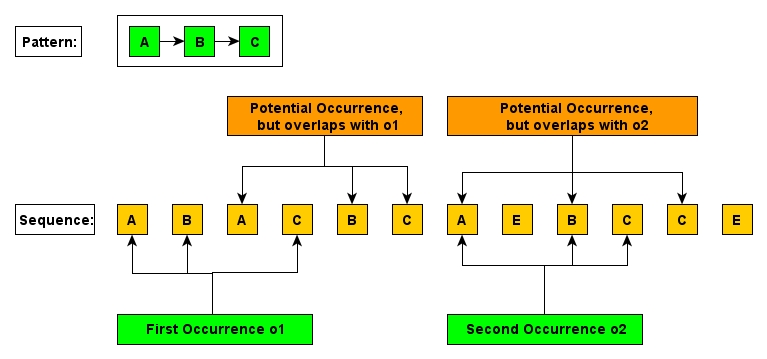
\includegraphics[width=\textwidth]{nonOverlappingExample}
	\caption{An example sequence that shows how occurrences of episode patterns can overlap. Two non-overlapping occurrences are colored in green, whereas the orange occurrences would overlap with one of the green occurrences.}
	\label{fig_nonOverlappingExample}
\end{figure}

\begin{mydef}
\label{def_nonOverlappingFrequency}
\textbf{Episode Frequency - Non-Overlapping Occurrences based Definition} Given a seqeunce of events $S$ and an Episode $\alpha$, we define the non-overlapping occurrence based frequency $noo\_freq(\alpha )$ as cardinality of the largest set of non-overlapped occurrences of $\alpha$ in $S$ \cite{laxman2007fast}.
\end{mydef}


When looking at these definitions in comparison to the window based frequency definition it is not clear whether any of these is always superior to or more useful than the other since they have different properties. We mention them briefly:

\begin{itemize}
	\item The window based frequency counts an episode occurrence that is comprised of the same events in multiple windows. This might especially distort the count if the window duration is high and the events in the episode happen with minimal delay between them.
	\item The minimal occurrence based definition of frequency does not suffer from the problem of the previous point, as it only counts the windows that contain a candidate episode, that can not be reduced in duration.
	\item The window based definition has the advantage that it already incorporates a fixed duration during which episodes may occur, meaning there can not be episodes that stretch over a time period larger than the fixed window duration $w$. This might be beneficial for potential algorithms, since it reduces the search space for episodes. On top of that it is also closer to reality, since in many domains episodes happen within a small time window.
	\item The non-overlapping occurrence based frequency seems to offer the fastest counting algorithm of all three definitions \cite{laxman2007fast}. However when incorporating expiry times for serial episodes some of this advantage gets lost \cite{laxman2006discovering}. Additionally previous literature has not yet identified an efficient algorithm to count non-overlapped occurrences of parallel episodes with expiry times. 
\end{itemize}

\section{Candidate Generation}
\label{sec_candidateGen}
Most previous work generates candidates for serial and parallel episodes separately, using a levelwise approach for both cases. The candidate generation procedure presented below was originally specified by Manila et al. \cite{mannila1997discovery}. A more detailed explanation can be found in Laxman's PHD thesis \cite{laxman2006discovering}. \newline
We first consider the case for parallel episodes. Given $F_k$ as the set of all frequent parallel episodes of length $k$ we can generate the candidate parallel episodes $C_{k+1}$ of length $k+1$ by doing the following:

\begin{enumerate}
	\item Represent each candidate $\alpha \in F_k$ as a lexicographically sorted array of length $k$.
	\item For each unordered pair $(\alpha , \beta )$, $\alpha ,\beta \in F_k$ where $\alpha$ and $\beta$ share the same first $k-1$ nodes, generate candidate $\gamma$ by copying $\alpha$ and appending $\beta [k]$.
\end{enumerate}

For example the two frequent parallel episodes $A \| A \| B$ and $A \| A \| C$ will generate the candidate $A \| A \| B \| C$. \newline
The same procedure can be applied to serial episodes, except that
\begin{itemize}
	\item we do not order lexicographically, instead the serial episodes remain in the array in their natural order
	\item each pair $(\alpha , \beta )$ with the same properties as above now generates two candidates:
	\begin{itemize}
		\item $\gamma{_1}$ by copying $\alpha$ and appending $\beta [k]$.
		\item $\gamma{_2}$ by copying $\beta$ and appending $\alpha [k]$.
	\end{itemize}
\end{itemize}

Thus the two frequent serial episodes $A \rightarrow A \rightarrow B$ and $A \rightarrow A \rightarrow C$ will now generate the two candidates $A \rightarrow A \rightarrow B \rightarrow C$ and $A \rightarrow A \rightarrow C \rightarrow B$. \newline
Since the mining of composite episodes has not received much attention, it is unsurprising that there little related work that mentions candidate generation strategies for these general types of episodes. For a more strict definition of composite episodes which only includes sequences of parallel episodes, Baumgarten et al. use a tree growth strategy to generate candidates for composite episodes \cite{baumgarten2003tree}. 

\section{Pattern Explosion}
\label{sec_PatternExplosion}
The term pattern explosion is often used to refer to the common problem of pattern mining algorithms of discovering many more patterns than can be processed (either by humans or automatically). This problem is potentially worse in episode mining than it is for classical frequent itemset mining, since the potential number of patterns is higher. Surprisingly, there is a notable absence of formulas for the number of episode patterns given a certain length or alphabet size in literature. It is however useful to have such formulas in order to have a rough idea just how many patterns may exist, since this may help in choosing appropriate support values. For parallel and serial episodes the combinatorial arguments are rather straightforward. Let $|\Sigma| = n$ be the size of the event alphabet. For the classical case of frequent itemset mining (with $\Sigma$ being the set of all items) the number of possible itemsets $N_I(n)$ is the size of the powerset of $\Sigma$:

\begin{equation}
	N_I(n) = 2^n
\end{equation}

Since events of the same type can occur multiple times in episodes, the number of episode patterns is not only dependent on the alphabet size $n$ but also the maximal length of patterns $m$. This means that in contrast to itemsets, episodes can have a higher length than the cardinality of the event alphabet $n$. The number of parallel episodes $N_P(n,m)$ can be calculated in the following way:

\begin{equation}
	N_P(n,m) = \sum_{i=1}^m {{n+i-1}\choose{n-1}}
\end{equation}

The argument is simple: For each length $i$ we draw $i$ events from an urn of size $n$ (which is $\Sigma$) with replacement, but without being interested in the order, which leads to exactly ${n+i-1}\choose{n-1}$ possibilities. To get all patterns up to length $m$, we simply sum up the individual terms. The number of serial episodes $N_S(n,m)$ can be calculated in the following way:

\begin{equation}
	N_S(n,m) = \sum_{i=1}^m n^i
\end{equation}

Serial episodes are formed in the same way, except that now the order matters, which means that this is equal to the problem of drawing $i$ events from an urn of size $n$ with replacement with being interested in the order, which means that there are $n^i$ combinations. Once again we sum over all lengths to obtain the complete number of patterns. \\
Such a formula is more difficult to find for composite episodes, since the different orderings and number of orderings are dificult to enumerate. In their paper about mining composite episodes Baathorn et al. \cite{bathoorn2007finding} provide a formula for the number of composite episodes $N_C(n,m)$:

\begin{equation}
\label{eq_numComposite}
	N_C(n,m) = \sum_{i=1}^m (2^n -1)^i
\end{equation}

However as discussed in section \ref{sec_basicEpisodeDefinitions} they define composite episodes as sequences of sets, which does not include all composite episodes according to definition \ref{def_compositeEpisodes}. This means that the number of composite episodes according to definition \ref{def_compositeEpisodes} is even higher than the one given by equation \ref{eq_numComposite}. \\
In order to get an idea of how the number of parallel and serial episode patterns develops, figure \ref{fig_patternExplosion} plots the values for a few alphabet sizes. Since this thesis only uses parallel and serial episodes, the number composite episodes is not depicted in the graph.

\begin{figure}[h]
	\centering
  	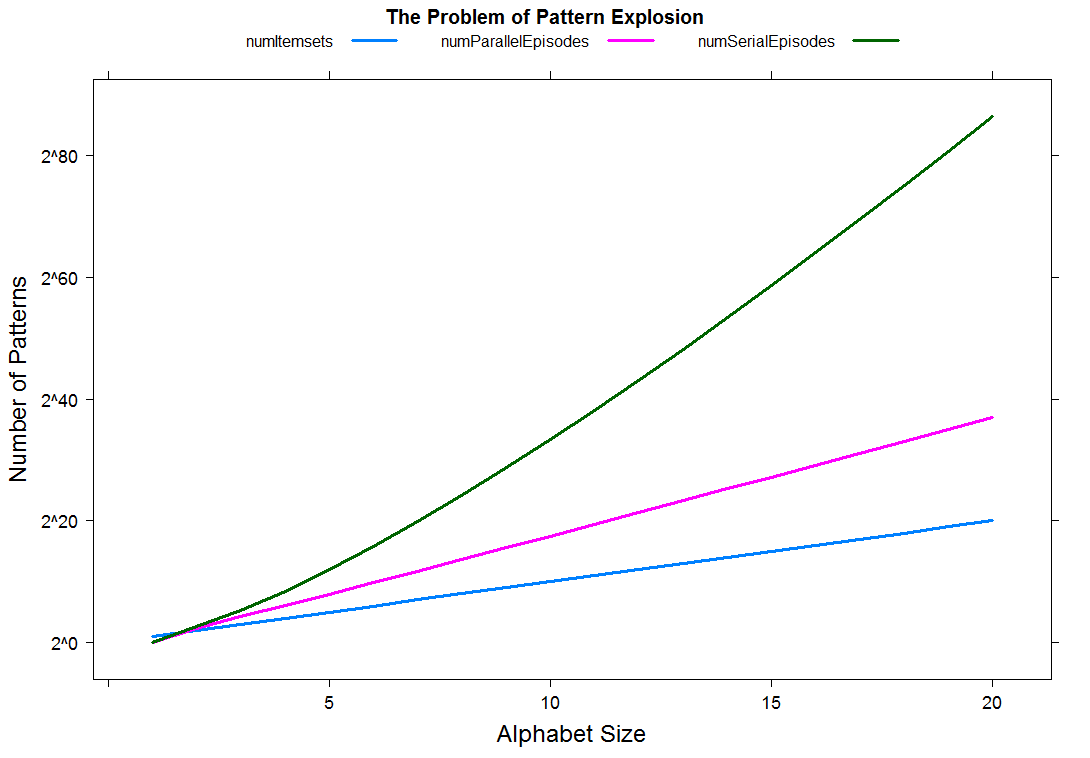
\includegraphics[width=0.75\textwidth]{patternExplosion}
	\caption{Number of patterns for Different Alphabet sizes. For each observation in this plot the maximal length of the episode patterns $m$ was set to the same value as the alphabet size to allow for a comparison with the number of frequent itemsets.}
	\label{fig_patternExplosion}
\end{figure}

Note that the scale of the y-axis is logarithmic, which shows that the number of possible episode patterns greatly exceeds the number of possible itemsets. This is practical information when choosing support thresholds for episode pattern mining algorithms, 